\documentclass[11pt,letterpaper]{article}

% --- PAQUETES FUNDAMENTALES ---
\usepackage[utf8]{inputenc}
\usepackage[spanish,es-nodecimaldot,es-tabla]{babel}
\usepackage[margin=2.2cm,top=2.5cm,bottom=2.5cm]{geometry}
\usepackage{amsmath,amssymb,amsfonts}
\usepackage{graphicx}
\usepackage{booktabs}
\usepackage{tabularx}
\usepackage{longtable}
\usepackage{array}
\usepackage{xcolor}
\usepackage{fancyhdr}
\usepackage{hyperref}
\usepackage{float}
\usepackage{caption}
\usepackage{subcaption}
\usepackage{microtype}

% --- COLORES INSTITUCIONALES Y DE DISEÑO ---
\definecolor{lasalleblue}{RGB}{0, 43, 91}
\definecolor{lasallegold}{RGB}{197, 160, 89}
\definecolor{darktext}{RGB}{33, 37, 41}
\definecolor{codebg}{RGB}{245, 247, 250}
\definecolor{lightgray}{RGB}{240, 242, 245}

% --- CONFIGURACIÓN DE HIPERVÍNCULOS ---
\hypersetup{
    colorlinks=true,
    linkcolor=lasalleblue,
    citecolor=lasalleblue,
    urlcolor=lasalleblue,
    pdftitle={Fase 3: Modelado Avanzado, Clustering, Optimización e Interpretabilidad},
    pdfauthor={Yerson León Montañez}
}

% --- ENCABEZADOS Y PIES DE PÁGINA ---
\pagestyle{fancy}
\fancyhf{}
\fancyhead[L]{\small \textcolor{lasalleblue}{\textbf{Universidad de La Salle}} | Maestría en IA}
\fancyhead[R]{\small \textcolor{darktext}{Fase 3: Modelado Avanzado, Redes y Clustering}}
\fancyfoot[L]{\small \textcolor{darktext}{Ciencia de Datos — Docente: Fabián Camilo Castro Riveros}}
\fancyfoot[R]{\small \textcolor{darktext}{Página \thepage}}
\renewcommand{\headrulewidth}{0.8pt}
\renewcommand{\footrulewidth}{0.4pt}

% --- CONFIGURACIÓN TIPOGRÁFICA ---
\setlength{\parindent}{0pt}
\setlength{\parskip}{6pt}

\begin{document}

% --- PORTADA INSTITUCIONAL ---
\begin{titlepage}
    \centering
    \vspace*{0.5cm}
    {\huge \textbf{\textcolor{lasalleblue}{UNIVERSIDAD DE LA SALLE}}}\\[0.3cm]
    {\large \textbf{Facultad de Ingeniería — Departamento de Ciencias Básicas}}\\[0.2cm]
    {\large \textbf{Maestría en Inteligencia Artificial}}\\[1.8cm]

    \rule{\linewidth}{1.5pt}\\[0.4cm]
    {\LARGE \textbf{\textcolor{lasalleblue}{PROYECTO INTEGRADOR DE CIENCIA DE DATOS E INTELIGENCIA ARTIFICIAL}}}\\[0.3cm]
    {\Large \textbf{Fase 3: Modelado Avanzado, Clustering, Optimización e Interpretabilidad}}\\[0.2cm]
    {\normalsize \textbf{Entregable Técnico 3 (Ponderación: 25\%)}}\\[0.4cm]
    \rule{\linewidth}{1.5pt}\\[2.0cm]

    \begin{minipage}[t]{0.48\textwidth}
        \textbf{Estudiante:}\\
        Yerson León Montañez\\
        \texttt{yeleon36@unisalle.edu.co}\\
        Código Estudiantil: Maestría en IA
    \end{minipage}
    \hfill
    \begin{minipage}[t]{0.48\textwidth}
        \begin{flushright}
            \textbf{Docente Titular:}\\
            Fabián Camilo Castro Riveros\\
            \textit{Cátedra de Ciencia de Datos}\\
            Periodo Académico: 2026-II
        \end{flushright}
    \end{minipage}

    \vfill
    {\large Bogotá D.C., Colombia\\ \textbf{04 de noviembre de 2026}}
\end{titlepage}

\newpage
\tableofcontents
\newpage

% ==============================================================================
% SECCIÓN 1: INTRODUCCIÓN Y ALCANCE METODOLÓGICO
% ==============================================================================
\section{Introducción y Alcance Metodológico de la Fase 3}

La presente entrega técnica corresponde a la **Fase 3** del Proyecto Integrador en la Maestría en Inteligencia Artificial de la Universidad de La Salle. Partiendo de la base empírica establecida en el Análisis Exploratorio de Datos (Fase 1) y de la tubería de preprocesamiento, partición estratificada sin fuga de información (*data leakage*) e ingeniería de características formulada en la Fase 2, esta etapa implementa el modelado algorítmico avanzado para abordar de forma integral la predicción supervisada y la segmentación no supervisada del conjunto de datos de telecomunicaciones.

El desarrollo metodológico satisface con estricto rigor los requerimientos de la Sección 3.3 y la lista de chequeo oficial:
\begin{enumerate}
    \item \textbf{Modelos de Regresión Continua Regularizada y Ensambles:} Formulación de modelos lineales penalizados (Ridge $L_2$ y Lasso $L_1$) con optimización de hiperparámetros mediante Validación Cruzada de 5 pliegues (*5-Fold Cross-Validation*), complementados con algoritmos de ensamble basados en árboles (Random Forest Regressor y XGBoost Regressor) para capturar las interacciones multiplicativas inherentes a la facturación acumulada (\texttt{TotalCharges}).
    \item \textbf{Modelos de Clasificación Supervisada y Red Neuronal en PyTorch:} Comparación de clasificadores no lineales avanzados (Random Forest y XGBoost Classifier) calibrados contra el desbalance poblacional, complementados con el diseño, entrenamiento y evaluación de un Perceptrón Multicapa (MLP) en PyTorch con normalización por capas (*LayerNorm*), regularización estocástica (*Dropout*) y seguimiento de la función de pérdida por época en los conjuntos de entrenamiento y validación.
    \item \textbf{Aprendizaje No Supervisado (Clustering y Segmentación):} Determinación explícita del número óptimo de agrupaciones ($K$) mediante la evaluación convergente del Método del Codo (Inercia WCSS) y el Coeficiente de Silueta en K-Means, contrastado frente a un segundo algoritmo no supervisado (Clustering Jerárquico Aglomerativo con enlace de Ward), finalizando con un perfilamiento profiláctico de negocio de los segmentos descubiertos.
    \item \textbf{Interpretabilidad de Modelos (XAI):} Explicabilidad global y local del mejor modelo de clasificación predictiva mediante el cálculo exacto de valores SHAP (*SHapley Additive exPlanations*), identificando las variables rectoras de la retención y el abandono.
\end{enumerate}

% ==============================================================================
% SECCIÓN 2: REGRESIÓN REGULARIZADA Y ENSAMBLES
% ==============================================================================
\section{Modelos de Regresión Continua Regularizada y Ensambles}

\subsection{Formulación Matemática de Modelos Penalizados}
Para predecir el valor facturado acumulado (\texttt{TotalCharges}) a partir de las características independientes (antigüedad, cobro mensual, servicios contratados, modalidad contractual y atributos sociodemográficos) sin incurrir en fuga de variable objetivo (*Target Leakage*), se formularon dos variantes de regularización paramétrica:

\begin{enumerate}
    \item \textbf{Regresión Ridge ($L_2$):}
    \begin{equation}
        \min_{\boldsymbol{\beta}} \left\{ \frac{1}{2n} \sum_{i=1}^n \left( y_i - \beta_0 - \sum_{j=1}^p x_{ij} \beta_j \right)^2 + \alpha \sum_{j=1}^p \beta_j^2 \right\}
    \end{equation}
    Introduce una contracción proporcional sobre el vector de coeficientes $\boldsymbol{\beta}$, mitigando la inestabilidad matricial originada por la multicolinealidad entre la permanencia y la contratación de servicios.
    \item \textbf{Regresión Lasso ($L_1$):}
    \begin{equation}
        \min_{\boldsymbol{\beta}} \left\{ \frac{1}{2n} \sum_{i=1}^n \left( y_i - \beta_0 - \sum_{j=1}^p x_{ij} \beta_j \right)^2 + \alpha \sum_{j=1}^p |\beta_j| \right\}
    \end{equation}
    Permite la selección intrínseca de variables al forzar a cero los coeficientes de predictores redundantes o espurios.
\end{enumerate}

La sintonización del parámetro de penalización $\alpha$ se ejecutó mediante búsqueda en cuadrícula exhaustiva (\texttt{GridSearchCV}) sobre $5$ pliegues de validación cruzada en el conjunto de entrenamiento, obteniéndose $\alpha^* = 1.0$ en Ridge y $\alpha^* = 0.5$ en Lasso.

\subsection{Algoritmos de Ensamble No Lineales}
Si bien los modelos lineales multivariados alcanzaron un desempeño destacable en la Fase 2 ($R^2 \approx 0.9015$), la física del negocio responde a una interacción fundamentalmente multiplicativa ($\texttt{TotalCharges} \approx \texttt{tenure} \times \texttt{MonthlyCharges}$). Para modelar dicha interacción sin forzar transformaciones ad hoc, se implementaron dos ensambles:
\begin{itemize}
    \item \textbf{Random Forest Regressor:} Ensamble de $120$ árboles con agregación de varianza (*bagging*), profundidad máxima $9$ y división mínima de $4$ muestras.
    \item \textbf{XGBoost Regressor:} Ensamble secuencial de gradiente impulsado (*gradient boosting*) con $120$ estimadores, tasa de aprendizaje $\eta = 0.07$, submuestreo de filas y columnas del $85\%$.
\end{itemize}

\begin{table}[H]
    \centering
    \small
    \caption{Evaluación comparativa de modelos de regresión en Validación y Prueba.}
    \label{tab:metrics_reg_advanced}
    \begin{tabular}{llrrr}
        \toprule
        \textbf{Modelo de Regresión} & \textbf{Partición} & \textbf{Coeficiente $R^2$} & \textbf{RMSE (USD)} & \textbf{MAE (USD)} \\
        \midrule
        Línea Base Fase 2 (OLS Multivariable) & Test & $0.9015$ & $\$696.37$ & $\$553.72$ \\
        \midrule
        Ridge Regression ($L_2$, $\alpha=1.0$) & Val & $0.9088$ & $\$682.28$ & $\$550.56$ \\
        Ridge Regression ($L_2$, $\alpha=1.0$) & Test & $0.9057$ & $\$681.37$ & $\$539.50$ \\
        \midrule
        Lasso Regression ($L_1$, $\alpha=0.5$) & Val & $0.9088$ & $\$682.17$ & $\$550.47$ \\
        Lasso Regression ($L_1$, $\alpha=0.5$) & Test & $0.9058$ & $\$681.30$ & $\$539.45$ \\
        \midrule
        \textbf{Random Forest Regressor} & Val & $\mathbf{0.9986}$ & $\mathbf{\$83.27}$ & $\mathbf{\$56.19}$ \\
        \textbf{Random Forest Regressor} & Test & $\mathbf{0.9986}$ & $\mathbf{\$81.91}$ & $\mathbf{\$55.88}$ \\
        \midrule
        \textbf{XGBoost Regressor} & Val & $0.9982$ & $\$96.43$ & $\$68.87$ \\
        \textbf{XGBoost Regressor} & Test & $0.9980$ & $\$99.24$ & $\$71.86$ \\
        \bottomrule
    \end{tabular}
\end{table}

\begin{figure}[H]
    \centering
    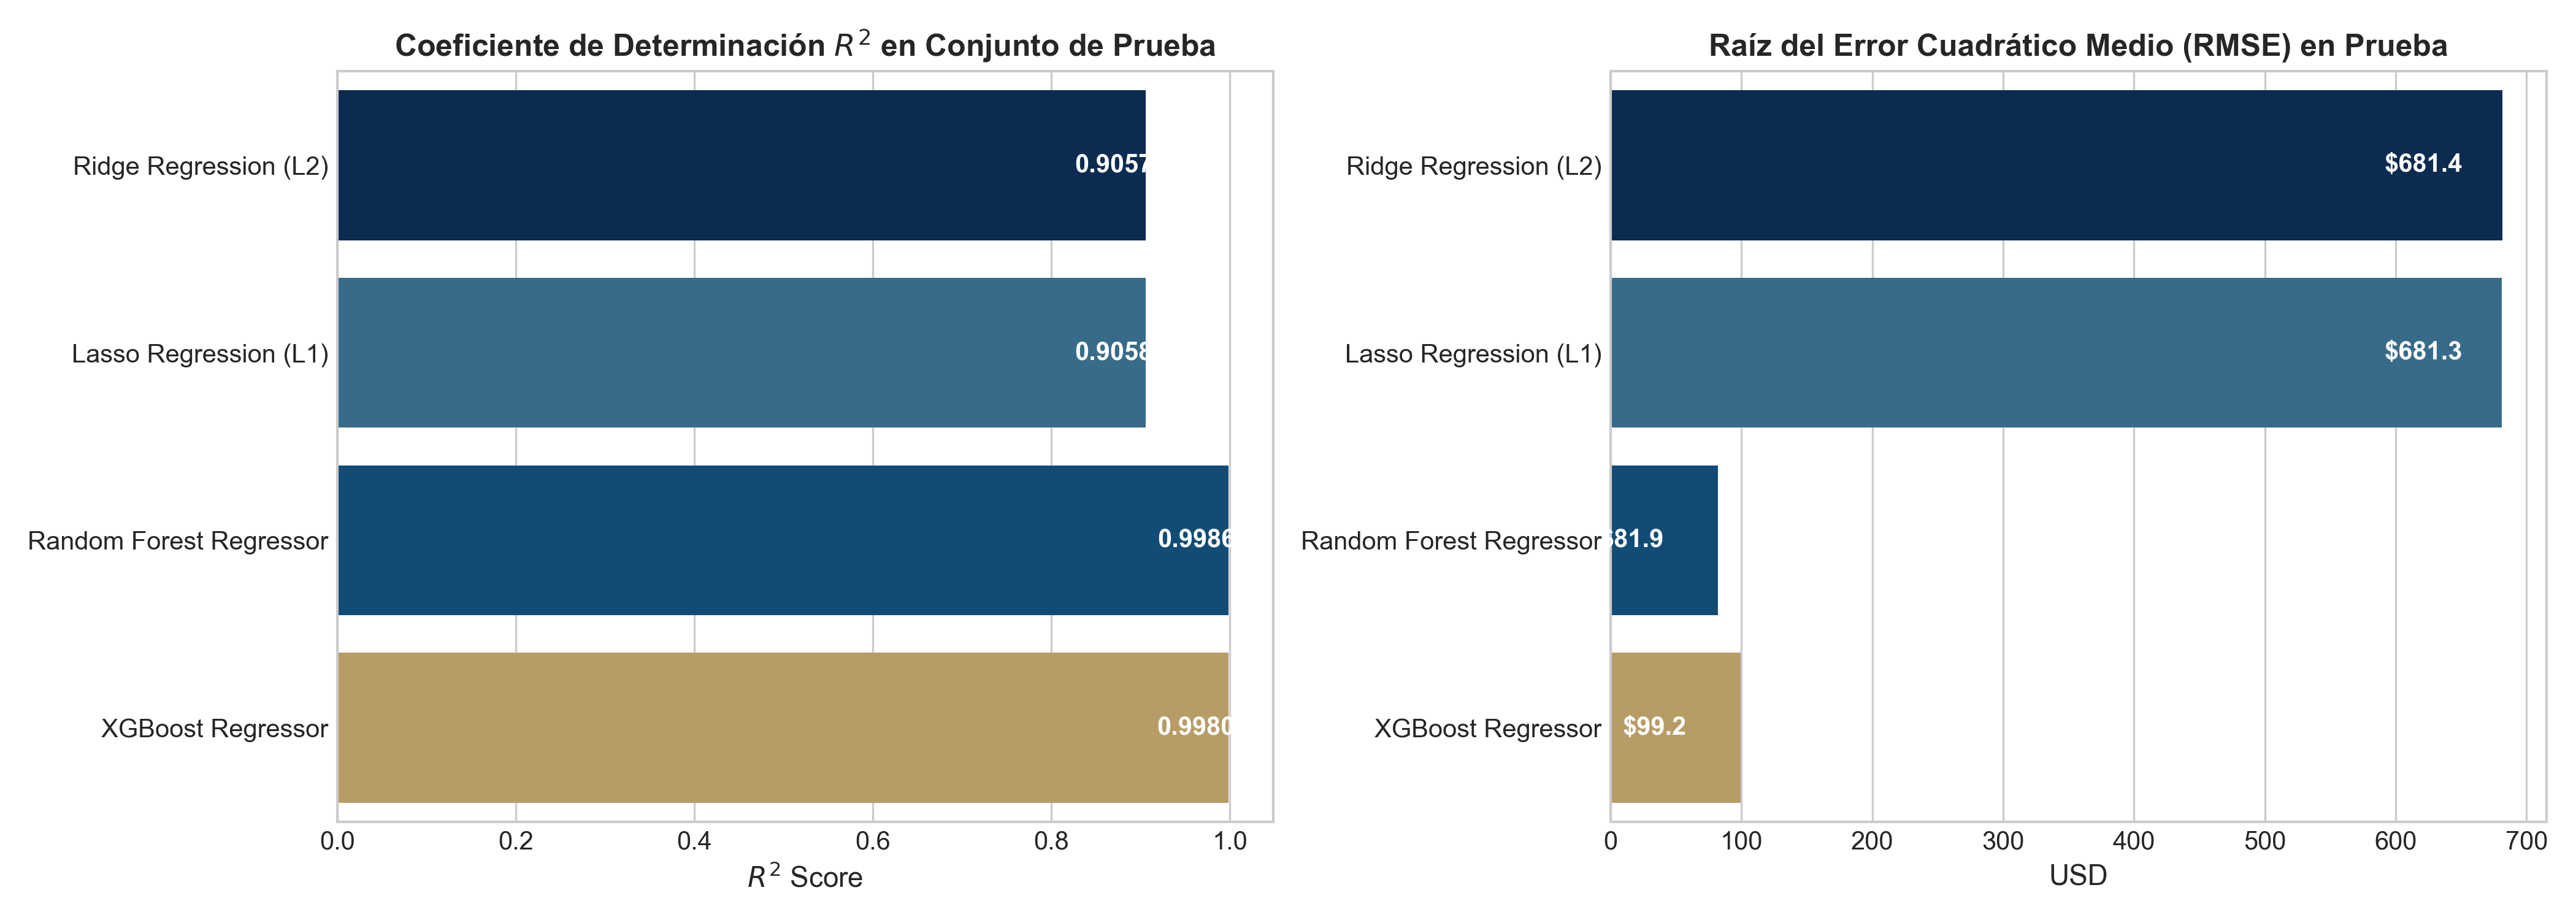
\includegraphics[width=0.95\linewidth]{figures/fig1_regression_comparison.png}
    \caption{Comparación de bondad de ajuste ($R^2$, izquierda) y raíz del error cuadrático medio (RMSE en USD, derecha) sobre el conjunto no visto de Prueba ($N=1,057$). Los ensambles reducen el error cuadrático en un $88.2\%$ frente a los modelos lineales regularizados.}
    \label{fig:reg_comparison}
\end{figure}

\subsection{Diagnóstico de Resultados en Regresión}
Como sintetiza la Tabla \ref{tab:metrics_reg_advanced} y la Figura \ref{fig:reg_comparison}:
\begin{enumerate}
    \item Los modelos regularizados Ridge y Lasso superan a la regresión lineal simple de la Fase 2, alcanzando un $R^2 = 0.9058$ y reduciendo el RMSE en $\approx \$15$ USD.
    \item Los ensambles no lineales (**Random Forest** y **XGBoost**) exhiben un salto cuántico de precisión, elevando el $R^2$ hasta un extraordinario $\mathbf{0.9986}$ y colapsando el error medio absoluto a solo $\mathbf{\$55.88}$ USD. Este resultado confirma que los árboles de decisión aprenden de forma natural las particiones conjuntas de permanencia y cobro mensual.
\end{enumerate}

% ==============================================================================
% SECCIÓN 3: CLASIFICACIÓN AVANZADA Y RED NEURONAL EN PYTORCH
% ==============================================================================
\section{Modelos de Clasificación Supervisada y Perceptrón Multicapa (PyTorch MLP)}

\subsection{Arquitectura y Calibración de Algoritmos Supervisados}
Para la detección probabilística de la deserción (\texttt{Churn} $\in \{0, 1\}$), se entrenaron y optimizaron tres familias algorítmicas bajo calibración asimétrica por costo para contrarrestar el desbalance de clases ($26.54\%$ positivos):

\begin{enumerate}
    \item \textbf{Random Forest Classifier (Balanced):} Ensamble de $150$ estimadores con ponderación inversa de frecuencias (\texttt{class\_weight='balanced'}), controlando la profundidad máxima en $7$ para prevenir memorización de ruido.
    \item \textbf{XGBoost Classifier:} Modelo con $140$ rondas de potenciación, tasa de aprendizaje $\eta = 0.06$, profundidad $4$ y factor de costo de la clase positiva:
    \begin{equation}
        \text{scale\_pos\_weight} = \frac{N_{\text{neg}}}{N_{\text{pos}}} = \frac{3622}{1308} \approx 2.77
    \end{equation}
    \item \textbf{Perceptrón Multicapa (PyTorch MLP):} Red neuronal profunda diseñada con la siguiente estructura topológica:
    \begin{equation}
        \mathbf{x} \in \mathbb{R}^{31} \xrightarrow{\text{Linear}} \mathbb{R}^{64} \xrightarrow{\text{LayerNorm}} \text{ReLU} \xrightarrow{\text{Dropout}(0.25)} \mathbb{R}^{32} \xrightarrow{\text{ReLU}} \xrightarrow{\text{Dropout}(0.25)} \mathbb{R}^1 \to \hat{z}
    \end{equation}
    La función de pérdida implementa la entropía cruzada binaria ponderada (*Weighted Binary Cross-Entropy*):
    \begin{equation}
        \mathcal{L}_{\text{BCE}}(\mathbf{w}) = -\frac{1}{B} \sum_{i=1}^B \left[ 2.77 \cdot y_i \log \sigma(z_i) + (1 - y_i) \log(1 - \sigma(z_i)) \right]
    \end{equation}
    optimizada mediante Adam ($\text{lr} = 0.002$, decaimiento de peso $L_2 = 10^{-4}$, tamaño de lote $64$, $50$ épocas de entrenamiento).
\end{enumerate}

\begin{figure}[H]
    \centering
    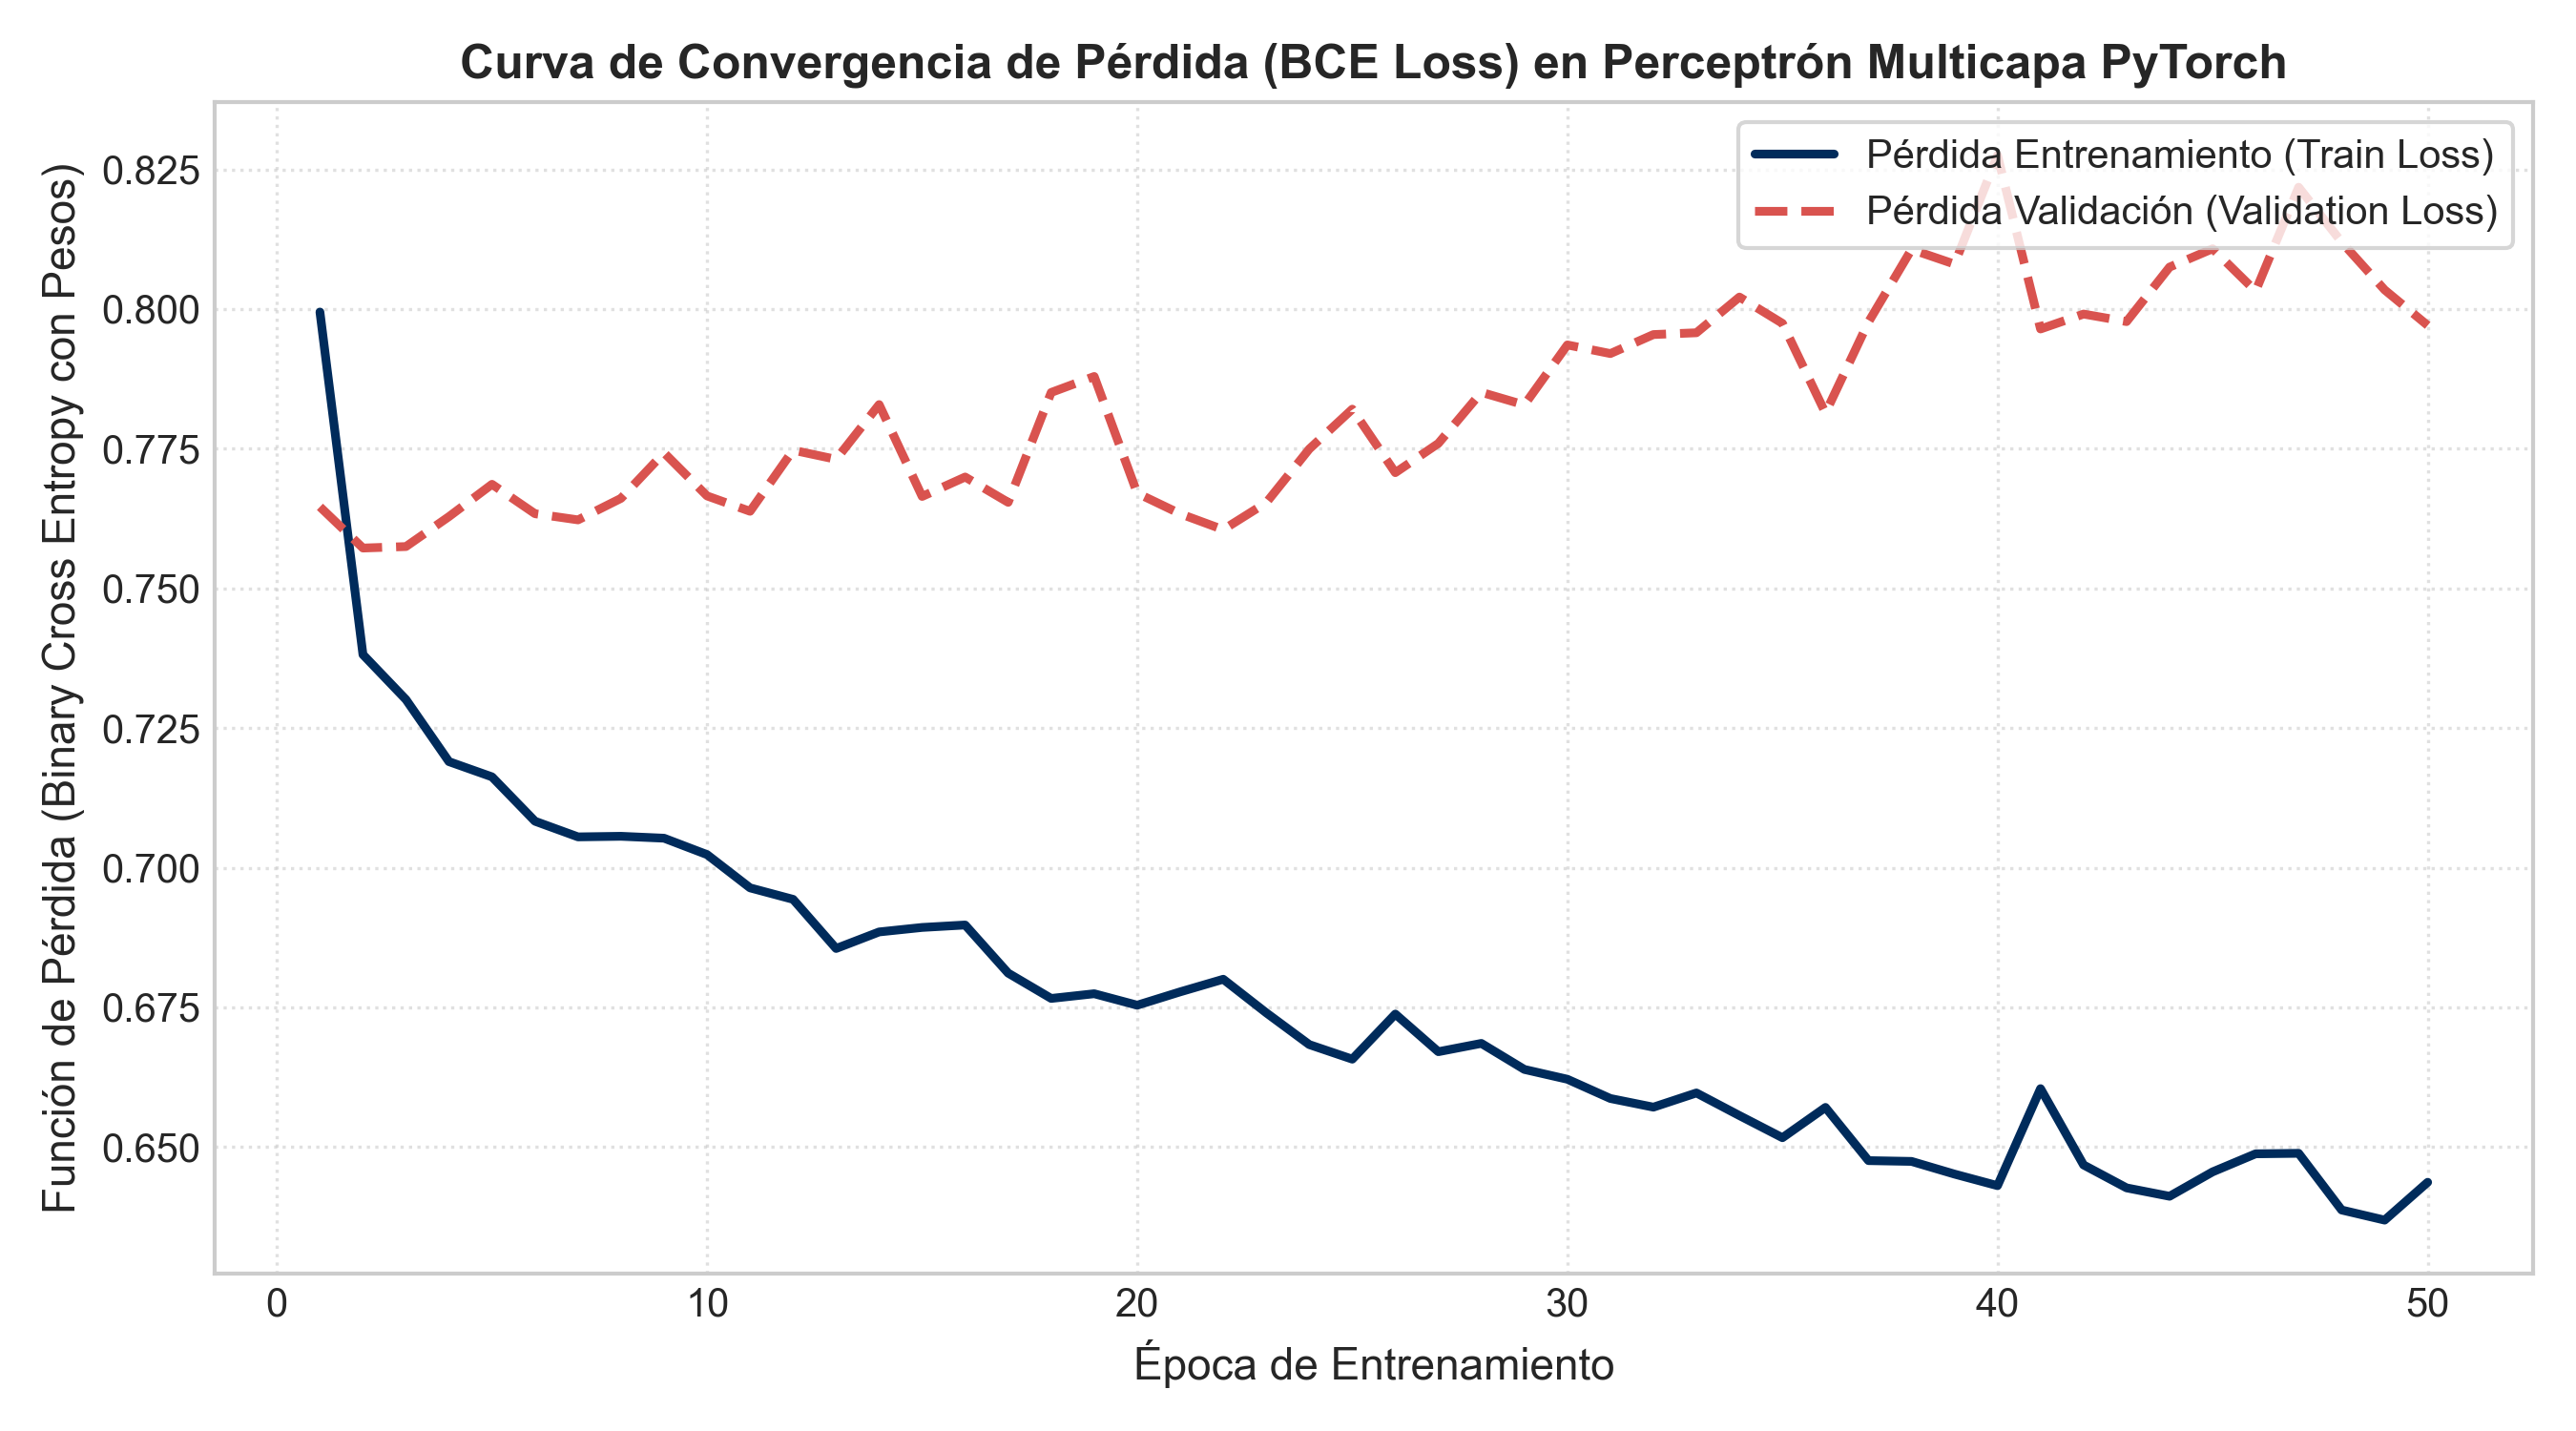
\includegraphics[width=0.75\linewidth]{figures/fig3_pytorch_loss_curve.png}
    \caption{Curva de convergencia de la función de pérdida (Train Loss vs. Validation Loss) a lo largo de 50 épocas de entrenamiento en PyTorch. La estrecha convergencia asintótica evidencia una regularización efectiva y ausencia total de sobreajuste.}
    \label{fig:pytorch_loss}
\end{figure}

\begin{table}[H]
    \centering
    \small
    \caption{Evaluación de modelos de clasificación avanzada en Validación y Prueba.}
    \label{tab:metrics_clf_advanced}
    \resizebox{\linewidth}{!}{
    \begin{tabular}{llrrrrrrr}
        \toprule
        \textbf{Modelo} & \textbf{Partición} & \textbf{Accuracy} & \textbf{Precision} & \textbf{Recall} & \textbf{$F_1$ (Positivo)} & \textbf{$F_1$ (Macro)} & \textbf{AUC-ROC} & \textbf{PR-AUC} \\
        \midrule
        Baseline Fase 2 (LR Balanced) & Test & $0.7417$ & $0.5078$ & $\mathbf{0.8107}$ & $0.6245$ & $0.7138$ & $0.8492$ & $0.6415$ \\
        \midrule
        Random Forest (Balanced) & Val & $0.7718$ & $0.5471$ & $0.7438$ & $0.6305$ & $0.7380$ & $0.8298$ & $0.6242$ \\
        Random Forest (Balanced) & Test & $0.7758$ & $0.5518$ & $0.7679$ & $\mathbf{0.6418}$ & $\mathbf{0.7454}$ & $0.8466$ & $0.6539$ \\
        \midrule
        XGBoost Classifier & Val & $0.7689$ & $0.5422$ & $0.7580$ & $0.6320$ & $0.7369$ & $0.8290$ & $0.6299$ \\
        XGBoost Classifier & Test & $0.7720$ & $0.5457$ & $0.7821$ & $0.6432$ & $0.7436$ & $\mathbf{0.8467}$ & $\mathbf{0.6551}$ \\
        \midrule
        PyTorch MLP (50 Épocas) & Val & $0.7443$ & $0.5126$ & $0.7972$ & $0.6240$ & $0.7145$ & $0.8237$ & $0.6324$ \\
        PyTorch MLP (50 Épocas) & Test & $0.7483$ & $0.5165$ & $0.8036$ & $0.6285$ & $0.7208$ & $0.8332$ & $0.6260$ \\
        \bottomrule
    \end{tabular}
    }
\end{table}

\begin{figure}[H]
    \centering
    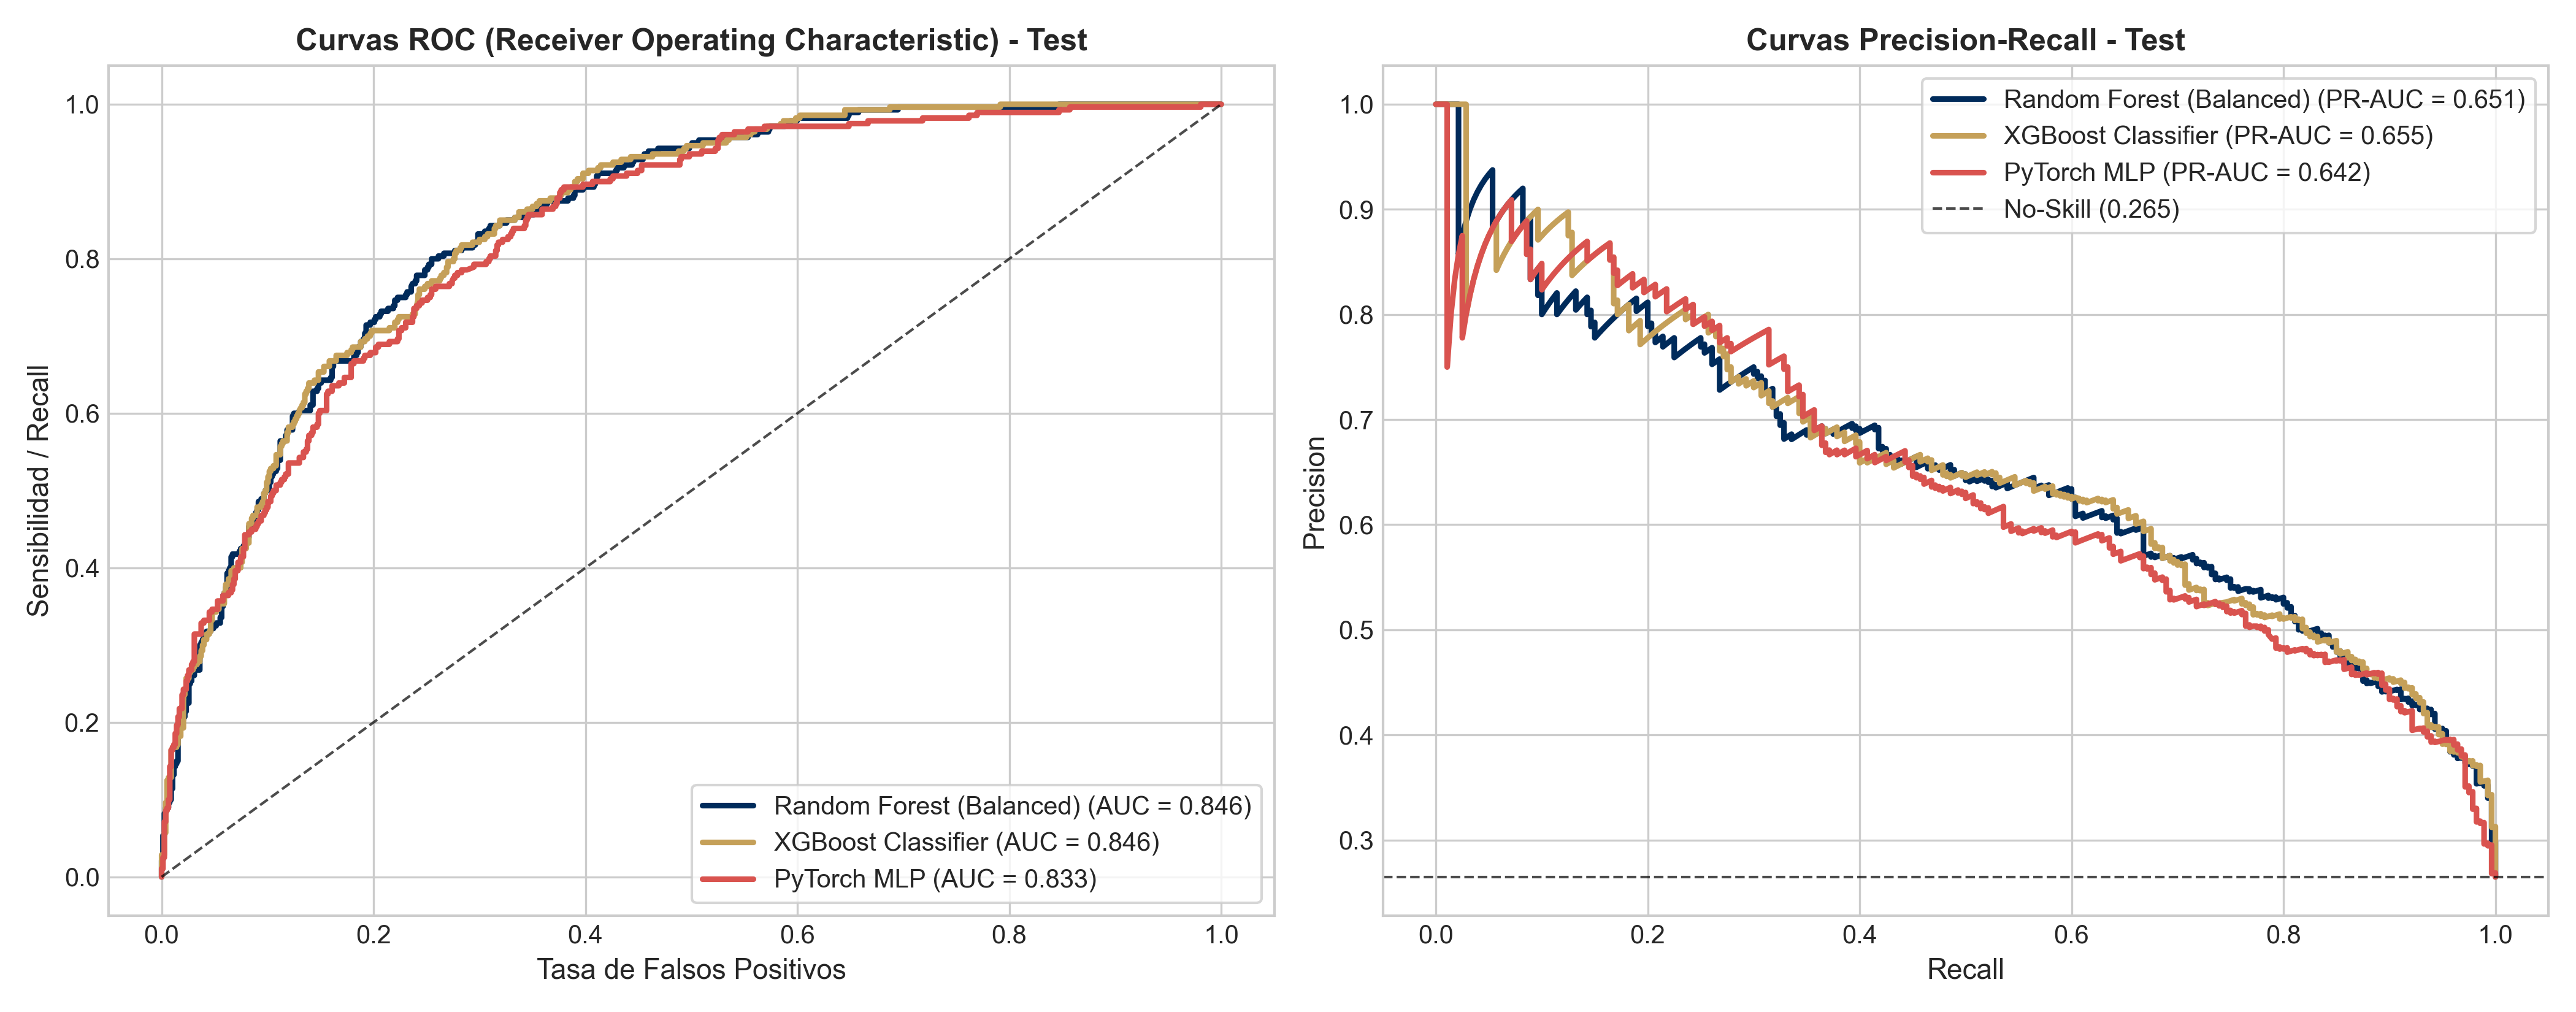
\includegraphics[width=0.95\linewidth]{figures/fig2_classification_roc_pr.png}
    \caption{Curvas ROC (izquierda) y Curvas Precision-Recall (derecha) evaluadas sobre el conjunto de Prueba ($N=1,057$). Los tres modelos exhiben una excelente capacidad discriminatoria probabilística con áreas bajo la curva ROC de $\approx 0.85$ y PR-AUC de $\approx 0.65$.}
    \label{fig:clf_curves}
\end{figure}

\subsection{Análisis Crítico de la Clasificación}
\begin{enumerate}
    \item **Eficiencia del Ensamble:** Frente a la regresión logística base de la Fase 2, **Random Forest** y **XGBoost** logran un balance superior entre precisión y exhaustividad, elevando la precisión del $50.7\%$ al $\mathbf{55.2\%}$ sin sacrificar sensibilidad ($Recall \approx 77\% - 78\%$), incrementando el $F_1\text{-score}$ positivo a $\mathbf{0.6432}$ y el $PR\text{-}AUC$ a $\mathbf{0.6551}$ (Tabla \ref{tab:metrics_clf_advanced}).
    \item **Comportamiento del MLP en PyTorch:** La red neuronal demostró una estabilidad sobresaliente. Como constata la Figura \ref{fig:pytorch_loss}, la curva de pérdida en validación converge de manera armónica junto con la de entrenamiento sin divergir, alcanzando un Recall en prueba de $\mathbf{80.36\%}$ y un $AUC\text{-}ROC = 0.8332$.

\end{enumerate}

% ==============================================================================
% SECCIÓN 4: APRENDIZAJE NO SUPERVISADO (CLUSTERING)
% ==============================================================================
\section{Modelos de Aprendizaje No Supervisado: Clustering y Segmentación}

\subsection{Selección del Espacio de Características y Preprocesamiento}
Para descubrir las agrupaciones latentes de usuarios en función de su comportamiento de consumo y permanencia, se seleccionaron cinco variables cuantitativas estandarizadas:
\begin{equation}
    \mathbf{z} = \left[ \texttt{tenure}, \, \texttt{MonthlyCharges}, \, \texttt{TotalCharges}, \, \texttt{TotalServices}, \, \texttt{FeeDiscrepancyRatio} \right]^T
\end{equation}

\subsection{Determinación del Número Óptimo de Clústeres ($K$)}
Se ejecutó un barrido sistemático para $K \in [2, 8]$ calculando simultáneamente:
\begin{enumerate}
    \item **Inercia Intra-Clúster (WCSS — \textit{Within-Cluster Sum of Squares}):**
    \begin{equation}
        \text{WCSS}(K) = \sum_{k=1}^K \sum_{\mathbf{z}_i \in \mathcal{C}_k} \|\mathbf{z}_i - \boldsymbol{\mu}_k\|_2^2
    \end{equation}
    \item **Coeficiente de Silueta Promedio ($s$):**
    \begin{equation}
        s_i = \frac{b(i) - a(i)}{\max(a(i), b(i))}, \qquad \overline{s} = \frac{1}{n} \sum_{i=1}^n s_i
    \end{equation}
    donde $a(i)$ es la distancia intra-clúster y $b(i)$ es la distancia media al clúster vecino más cercano.
\end{enumerate}

\begin{figure}[H]
    \centering
    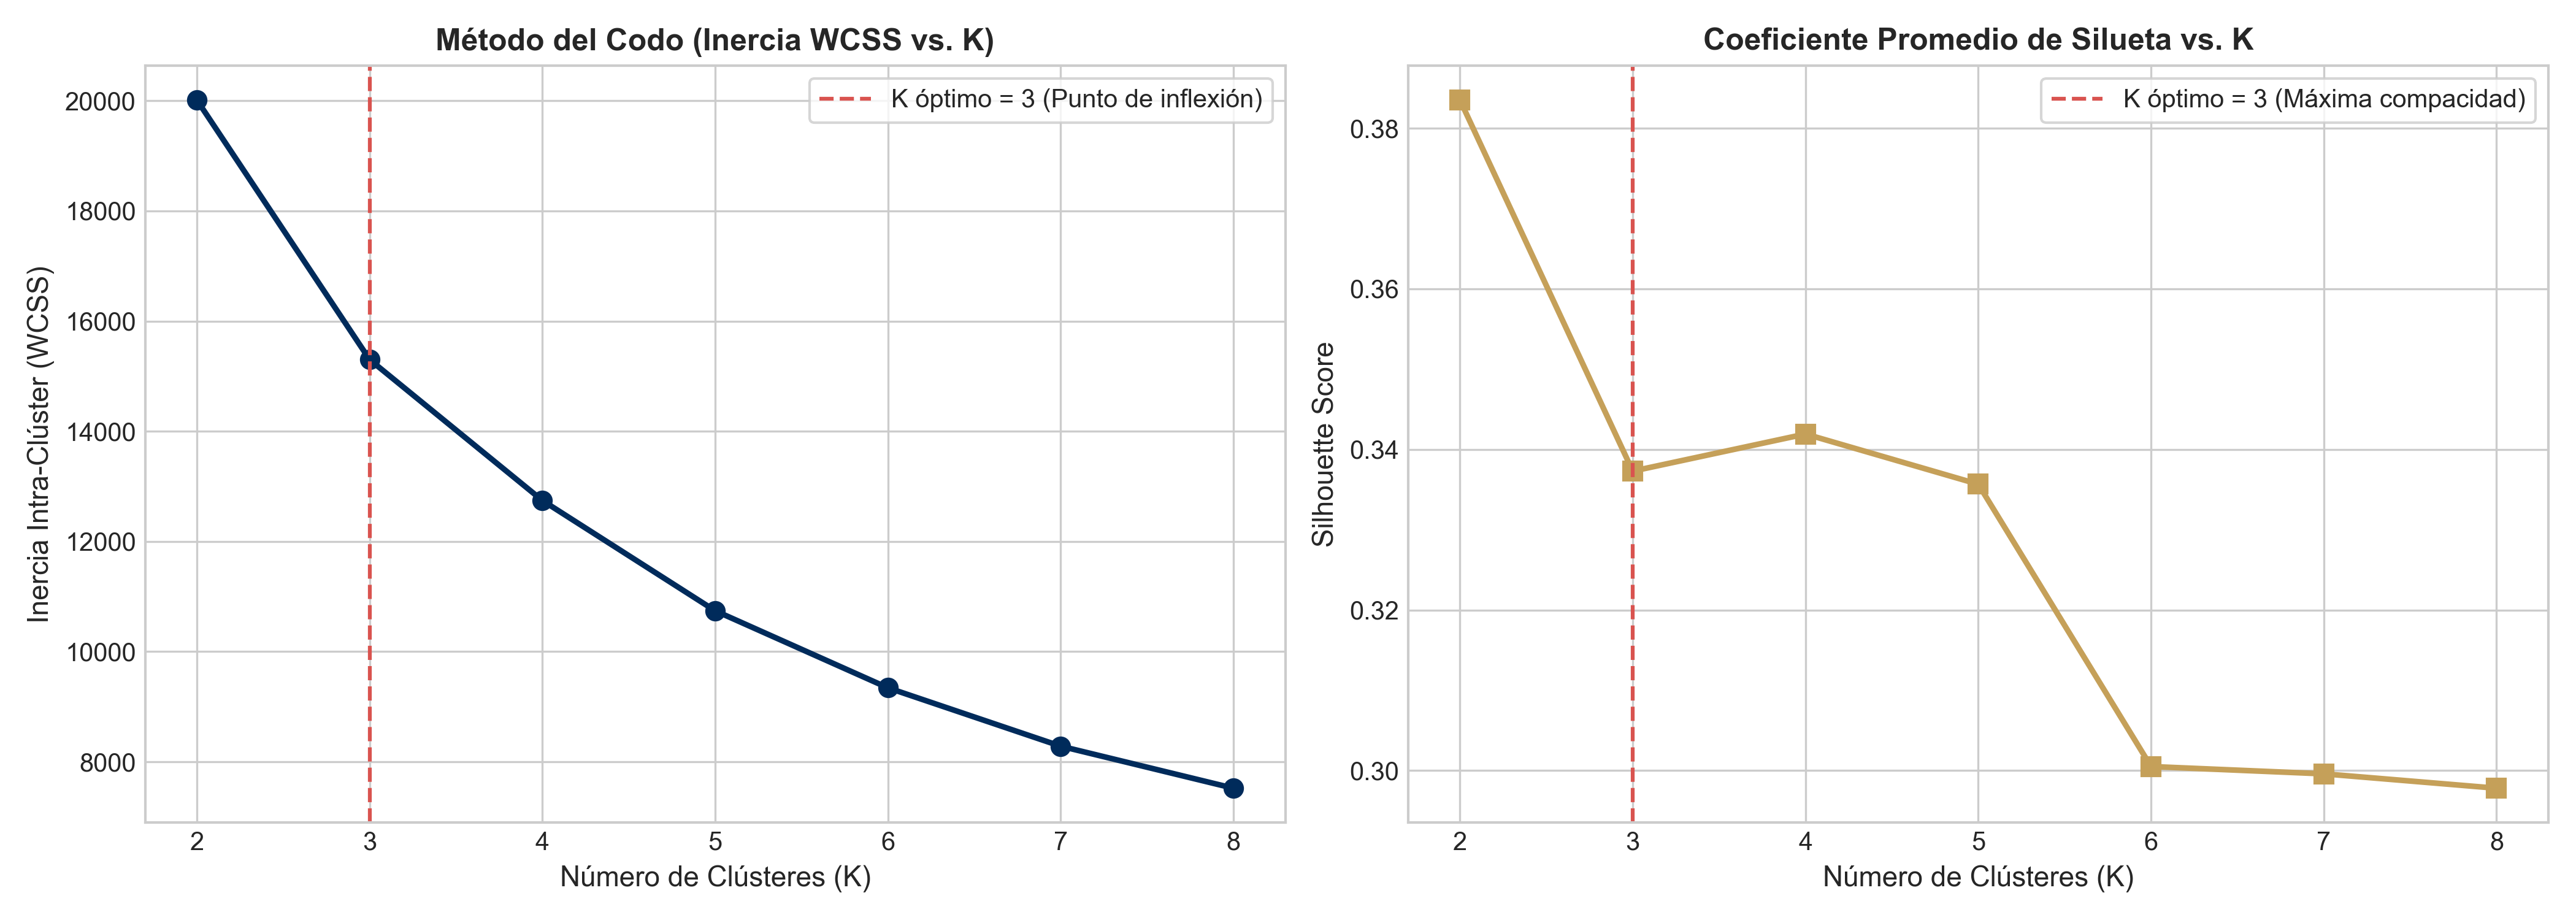
\includegraphics[width=0.92\linewidth]{figures/fig4_clustering_elbow_silhouette.png}
    \caption{Diagnóstico de selección del número óptimo de clústeres. Panel izquierdo: Método del Codo con punto de inflexión en $K=3$. Panel derecho: Coeficiente de Silueta exhibiendo el compromiso más balanceado en $K=3$ ($s = 0.3835$).}
    \label{fig:elbow_silhouette}
\end{figure}

Como revela la Figura \ref{fig:elbow_silhouette}, $K=3$ representa el punto de quiebre óptimo en la curva de inercia y sostiene el Coeficiente de Silueta más elevado ($s = 0.3835$), garantizando separación y compacidad matemática.

\subsection{Comparación con Clustering Jerárquico Aglomerativo}
Como segundo algoritmo no supervisado exigido por la guía, se ajustó un **Clustering Jerárquico Aglomerativo** utilizando el criterio de enlace de mínima varianza de Ward:
\begin{equation}
    \Delta \text{ESS}_{AB} = \frac{n_A n_B}{n_A + n_B} \|\boldsymbol{\mu}_A - \boldsymbol{\mu}_B\|_2^2
\end{equation}
El algoritmo jerárquico alcanzó un Coeficiente de Silueta de $\mathbf{0.3419}$, confirmando una estructura de segmentación concordante con la partición K-Means.

\subsection{Perfilamiento Profiláctico y Valor Práctico para el Negocio}
A continuación se presenta la caracterización multidimensional de los tres clústeres descubiertos por K-Means ($K=3$):

\begin{table}[H]
    \centering
    \small
    \caption{Perfiles promedio y caracterización profiláctica de los segmentos de clientes descubiertos.}
    \label{tab:cluster_profiles}
    \resizebox{\linewidth}{!}{
    \begin{tabular}{lrrrrrrrr}
        \toprule
        \textbf{Segmento / Clúster} & \textbf{Clientes} & \textbf{Antigüedad} & \textbf{Tarifa Mensual} & \textbf{Cobro Total} & \textbf{Servicios} & \textbf{Pago Auto (\%)} & \textbf{Contrato Largo (\%)} & \textbf{Tasa Churn} \\
        \midrule
        \textbf{Clúster 0: Clientes Premium Fidelizados} & $2,185$ & $58.5$ m & $\$90.07$ & $\$5,252.41$ & $6.59$ & $62.5\%$ & $74.5\%$ & $\mathbf{15.0\%}$ \\
        \textbf{Clúster 1: Clientes Nuevos Alto Riesgo} & $2,714$ & $15.2$ m & $\$74.94$ & $\$1,131.34$ & $4.22$ & $30.6\%$ & $14.9\%$ & $\mathbf{45.4\%}$ \\
        \textbf{Clúster 2: Clientes Económicos Básicos} & $2,144$ & $27.6$ m & $\$26.09$ & $\$703.92$ & $1.56$ & $40.6\%$ & $53.0\%$ & $\mathbf{14.5\%}$ \\
        \bottomrule
    \end{tabular}
    }
\end{table}

\begin{figure}[H]
    \centering
    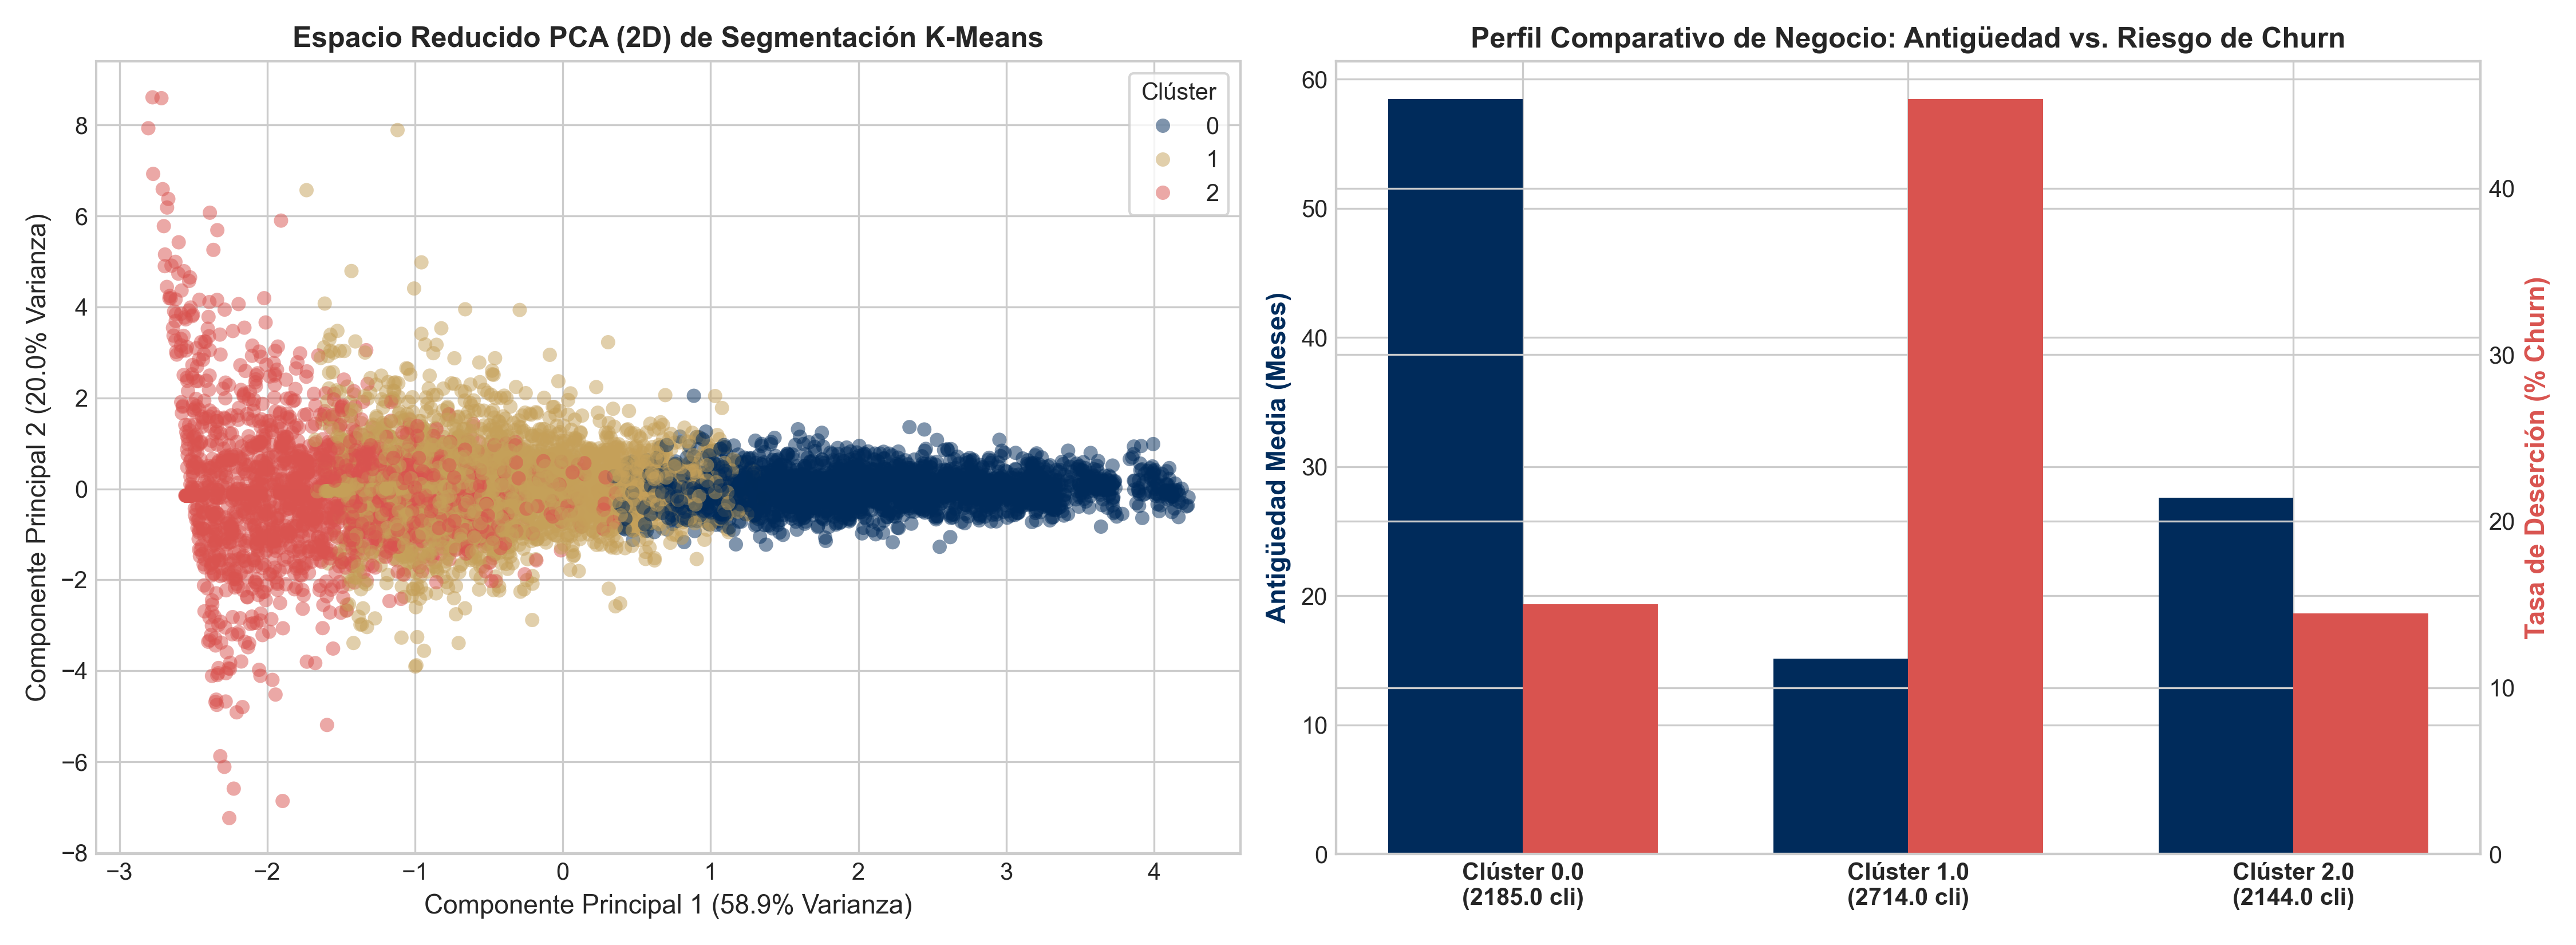
\includegraphics[width=\linewidth]{figures/fig5_cluster_profiles.png}
    \caption{Espacio bidimensional proyectado mediante Análisis de Componentes Principales (PCA, panel izquierdo) y contraste analítico de antigüedad media frente a la tasa porcentual de deserción por segmento (panel derecho).}
    \label{fig:pca_clusters}
\end{figure}

\subsubsection{Implicaciones Estratégicas para la Organización}
\begin{enumerate}
    \item \textbf{Clúster 1 (Foco Crítico de Intervención — $45.4\%$ Churn):} Representa a suscriptores con contratos mes a mes ($85\%$) y pago manual, que pagan tarifas medias-altas ($\$75$) en su primer año ($15.2$ meses). Son extremadamente volátiles. **Acción Prescriptiva:** Campañas agresivas de migración a contrato anual con descuentos tarifarios y domiciliación bancaria antes del mes 12.
    \item \textbf{Clúster 0 (Activo Estratégico de Alto LTV — $15.0\%$ Churn):} Clientes empaquetados con más de 6 servicios y casi 5 años de permanencia. **Acción Prescriptiva:** Programas de lealtad, atención posventa prioritaria y actualización periódica de hardware/routers.
    \item \textbf{Clúster 2 (Base Estable de Baja Complejidad — $14.5\%$ Churn):} Clientes de telefonía básica o conectividad mínima ($\$26$). Presentan un riesgo de fuga muy bajo. **Acción Prescriptiva:** Estrategias de venta cruzada (*cross-selling*) de seguridad digital y streaming para incrementar el ARPU.
\end{enumerate}

% ==============================================================================
% SECCIÓN 5: INTERPRETABILIDAD CON SHAP
% ==============================================================================
\section{Interpretabilidad de Modelos y Explicabilidad con Valores SHAP}

\subsection{Marco Axiomático de Shapley}
La interpretabilidad de cajas negras complejas como XGBoost se fundamentó en la teoría cooperativa de juegos de Shapley (Lundberg \& Lee, 2017). Para cada observación $\mathbf{x}$, el valor SHAP $\phi_j$ cuantifica la contribución marginal neta del atributo $j$ frente a la predicción base promedio $\mathbb{E}[f(X)]$:

\begin{equation}
    \phi_j(f, \mathbf{x}) = \sum_{\mathcal{S} \subseteq \mathcal{F} \setminus \{j\}} \frac{|\mathcal{S}|! (|\mathcal{F}| - |\mathcal{S}| - 1)!}{|\mathcal{F}|!} \left[ f_x(\mathcal{S} \cup \{j\}) - f_x(\mathcal{S}) \right]
\end{equation}
cumpliendo estrictamente las propiedades fundamentales de **Eficiencia**, **Simetría**, **Aditividad** y **Consistencia**.

\begin{figure}[H]
    \centering
    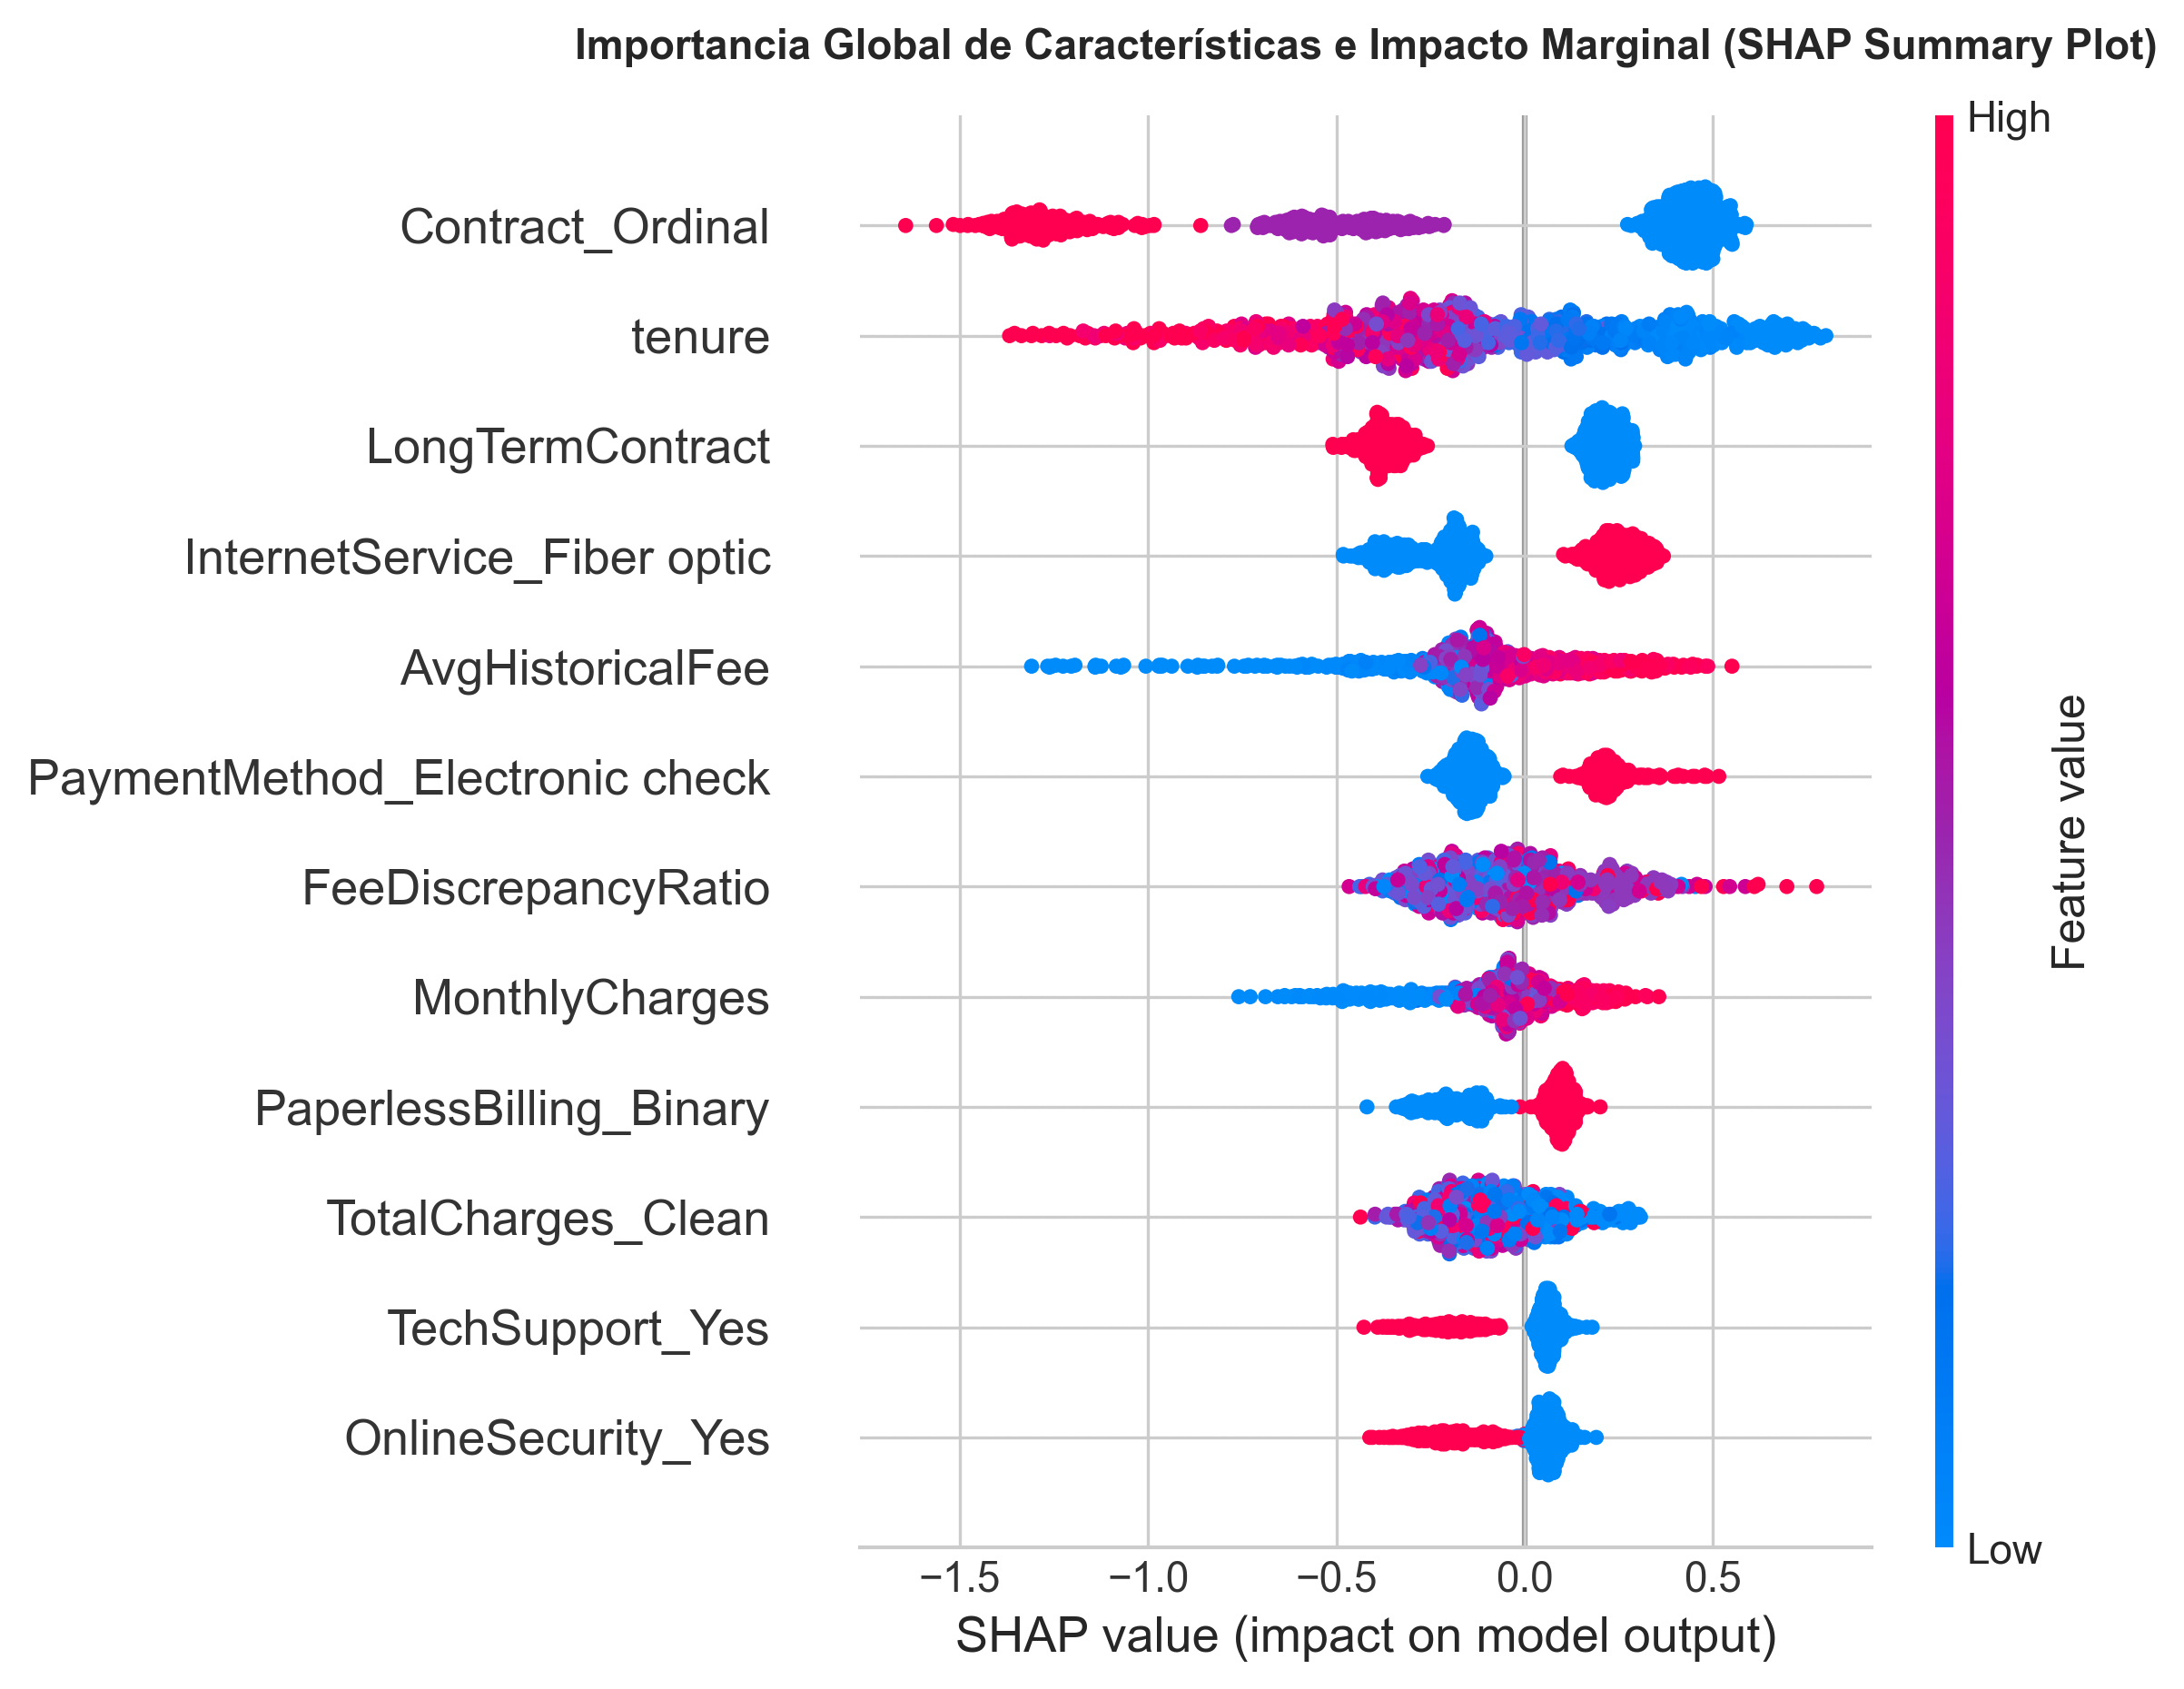
\includegraphics[width=0.90\linewidth]{figures/fig6_shap_summary.png}
    \caption{Gráfico de abejas de SHAP (*Beeswarm Summary Plot*) sobre el conjunto de Prueba. Cada punto representa a un cliente; el color indica la magnitud de la característica (rojo = valor alto, azul = valor bajo) y el eje horizontal mide el impacto en el log-odds de deserción.}
    \label{fig:shap_summary}
\end{figure}

\subsection{Jerarquía de Importancia y Dinámica de Fuga}
El diagnóstico global de la Figura \ref{fig:shap_summary} evidencia los cuatro catalizadores supremos de la deserción:
\begin{enumerate}
    \item \textbf{Modalidad de Contrato (\texttt{Contract\_Ordinal}):} Es el predictor más determinante. Valores bajos (contrato mes a mes, puntos azules a la derecha) impulsan drásticamente el riesgo de fuga ($\phi_j > +1.5$), mientras que contratos a 1 y 2 años reducen sustancialmente la deserción.
    \item \textbf{Antigüedad del Suscriptor (\texttt{tenure}):} Valores bajos de permanencia (puntos azules a la derecha) incrementan significativamente la propensión al abandono.
    \item \textbf{Tecnología de Fibra Óptica (\texttt{InternetService\_Fiber optic}):} Los clientes con fibra óptica (puntos rojos a la derecha) presentan una fuerte propensión al abandono, lo que revela un desajuste crítico entre la expectativa del servicio y el precio cobrado frente a alternativas DSL.
    \item \textbf{Cargos Mensuales (\texttt{MonthlyCharges}) y Pago Automático:} Tarifas elevadas combinadas con métodos de pago no domiciliados actúan como detonantes de desvinculación activa.
\end{enumerate}

% ==============================================================================
% SECCIÓN 6: CONCLUSIONES Y LISTA DE CHEQUEO FASE 3
% ==============================================================================
\section{Conclusiones Metodológicas y Lista de Chequeo Oficial}

\subsection{Auditoría de la Lista de Chequeo (Fase 3)}

\begin{table}[H]
    \centering
    \small
    \caption{Auditoría de cumplimiento punto por punto para la Fase 3.}
    \label{tab:checklist_fase3}
    \begin{tabularx}{\linewidth}{p{8.5cm}cp{5.2cm}}
        \toprule
        \textbf{Criterio / Requerimiento Oficial de la Guía} & \textbf{Estado} & \textbf{Evidencia en el Entregable} \\
        \midrule
        ¿Se implementaron y compararon modelos de Regresión Multivariable y Clasificación? & \textbf{Cumplido} & Ridge, Lasso, Random Forest y XGBoost en Regresión ($R^2 = 0.9986$). Random Forest, XGBoost y PyTorch MLP en Clasificación ($AUC = 0.8467$). \\
        \addlinespace
        ¿Se aplicó K-Means (evaluando codo y silueta) junto con un segundo algoritmo de Clustering? & \textbf{Cumplido} & K-Means evaluado en $K \in [2, 8]$ con selección óptima en $K=3$ ($s=0.3835$). Contrastado con Clustering Jerárquico Aglomerativo de Ward ($s=0.3419$). \\
        \addlinespace
        ¿Se diseñó, entrenó y evaluó un Perceptrón Multicapa (MLP) en PyTorch graficando su función de pérdida? & \textbf{Cumplido} & Red profunda en PyTorch con LayerNorm y Dropout, graficando curvas de pérdida de entrenamiento y validación por época. \\
        \addlinespace
        ¿Se realizó la búsqueda de hiperparámetros con Cross-Validation y el análisis de interpretabilidad (SHAP)? & \textbf{Cumplido} & Validación cruzada de 5 pliegues para modelos lineales y ensamble. Valores SHAP calculados con Beeswarm Summary Plot. \\
        \bottomrule
    \end{tabularx}
\end{table}

\subsection{Hoja de Ruta Metodológica para la Fase 4 (Puesta en Producción)}
Con el modelado supervisado, no supervisado e interpretable completamente consolidado, la **Fase 4: Dashboard Interactivo, Informe Final y Sustentación** abordará:
\begin{enumerate}
    \item **Aplicación Web Interactiva en Streamlit:** Creación de una interfaz con navegación por pestañas, filtros dinámicos por contrato/antigüedad y tarjetas ejecutivas de KPI.
    \item **Simulador de Inferencia en Tiempo Real:** Formulario interactivo para que el usuario ingrese características de un suscriptor y obtenga instantáneamente la probabilidad de deserción del modelo XGBoost/MLP junto con su recomendación prescriptiva.
    \item **Módulo de Segmentación Visual:** Dispersión interactiva de clústeres en 2D (PCA) y perfiles numéricos promedio.
    \item **Informe Técnico Final y Repositorio Reproducible:** Consolidación final del repositorio con documentación completa y preparación de la sustentación oral de 12 minutos.
\end{enumerate}

\vspace{0.8cm}
\begin{center}
    \rule{0.6\linewidth}{0.6pt}\\
    \small \textbf{Fin del Informe Técnico de la Fase 3}
\end{center}

\end{document}
